\section{Exploration by UCB bonus}
We cite Cai's \cite{cai2019provably} theoretical work on regret decomposition and the upper bound of model prediction error under linear MDP approximation. Then we introduce the Actor-Critic algorithm with UCB bonus in the context of deep neural networks.

\subsection{Regret Decomposition}
In \cite{cai2019provably} paper, an Optimistic Policy Optimization (OPPO) algorithm is proposed for the MDP with adversarial rewards and stochastic transition dynamics. The policy improvement step and the policy evaluation step can be briefly expressed as:
\begin{eqnarray}
    &&\pi_h^{k+1}(\cdot,\cdot)\propto \pi_h^k(\cdot,\cdot)\cdot \text{exp}\{\alpha\cdot Q_h^k(\cdot,\cdot)\}\\
    &&Q_h^k(\cdot,\cdot)\leftarrow r_h^k(\cdot,\cdot)+\mathbb{E}_{\hat{\mathbb{P}}(s'|\cdot,\cdot)}[V^k_{h+1}(s')]\\
    &&V^k_h(\cdot)\leftarrow \langle Q_h^k(\cdot,\cdot),\pi^k_h(\cdot,\cdot)\rangle
\end{eqnarray}


The regret of the OPPO algorithm can be de down into three terms:
\begin{equation}
    \begin{split}
        &\text{Regret}(T)=\sum_{k=1}^K(V_1^{\pi^*,k}(s^k_1)-V_1^{\pi^k,k}(s^k_1))\\
        &=\underbrace{\sum_{k=1}^K\sum_{h=1}^H\mathbb{E}_{\pi^*}[\langle Q^k_h(s_h,\cdot),\pi^*_h(\cdot|s_h)-\pi^k_h(\cdot|s_h) \rangle|s_1=s_1^k]}_{(i)}\\
        &+\underbrace{\mathcal{M}_{K,H,2}}_{(ii)}\\
        &+\underbrace{\sum_{k=1}^K\sum_{h=1}^H(\mathbb{E}_{\pi^*}[\iota_h^k(s_h,a_h)|s_1=s_1^k]-\iota_h^k(s_h^k,a_h^k))}_{(iii)}
    \end{split}\label{eq:regret}
\end{equation}

The term (i) is due to the adversarial reward. Since in each turn the reward function is selected by the adversary, the policy improvement step size needs to be selected carefully to avoid being too "extreme" or too "conservative". The term (ii) is a martingale which is associated with the stochastic transition dynamics.

We focus on the third item, where $\iota$ is the \textbf{model prediction error} which defined as:
\begin{equation}
\iota_h^k(s,a) = r_h^k(s,a) + \mathbb{E}_{\mathbb{P}_h(s'|s,a)}[V_{h+1}^k(s')] -Q_h^k(s,a)
\end{equation}
This term is because only limited historical data is used to update $Q$ by Bellman Equation, which results in the predict $Q$ differs from $r+\mathbb{E}_{\mathbb{P}(s'|s,a)}[V(s')]$ with real transition dynamics  $\mathbb{P}(s'|s,a)$. To bound the third term we need more assumptions on the property of MDP.

\subsection{Linear MDP Approximation}
To further analyze the bounds of the third term, the linear MDP approximation is introduced. We assume that the MDP is a linear MDP with feature mapping $\phi : \mathcal{S}\times \mathcal{A} \rightarrow \mathbb{R}^d$. That is there exist $d$ measures $\mu_h=(\mu_h^1,\cdots,\mu_h^d)\top$ on $\mathcal{S}$ and a vector $\theta_h^k \in \mathbb{R}^d$ such that:
\begin{align}
    \mathbb{P}_h(s'|s,a)&=\phi(s,a)^\top\mu_h(s')\\
    r_h^k(s,a)&=\phi(s,a)^\top\theta^k_h
\end{align}
Under the linear approximation, there exist vector $w_h^{\pi,k}\in\mathbb{R}^d$ for any policy $\pi$ such that:
\[Q_h^{\pi,k}(s,a) = r_h^k(s,a)+\phi(s,a)^\top w_h^{\pi,k}\]
The $w_h^{\pi,k}$ can be estimated by Least-Squares Temporal Difference (LSTD) method:

\begin{align}
    & \Lambda_h^k \leftarrow \sum_{k=1}^{K}\phi(s_h^k,a_h^k)\phi(s_h^k,a_h^k)^\top+\lambda\cdot I\\
    & w_h^k \leftarrow (\Lambda_h^k)^{-1}\sum_{k=1}^{K}\phi(s_h^k,a_h^k) V^k_{h+1}(s_{h+1}^k)\\
    & Q_h^k(s,a)\leftarrow r_h^k(s,a) + \phi(s,a)^\top w_h^k \label{eq:LSTD}
\end{align}
    
By add bonus $\beta[\phi(s,a)^\top(\Lambda_h^k)^{-1}\phi(s,a)]^{1/2}$ on right-side of Equation (\ref{eq:LSTD}) and select 
\[\beta=CdH\sqrt{\log(dT/\zeta)}\]
the regret term (iii)  in Equation (\ref{eq:regret}) is bounded by 
\[\text{Regret}(T) \leq 2C\sqrt{2d^3H^3T}\log(dT/\zeta)\]
with probability at least $1-\zeta/2$.

\subsection{Optimistic Actor-Critic}
So far we have introduced the results of Cai's article on the regret bound under the linear MDP approximation. To achieve a practical exploration strategy, we consider the context of function approximation via deep neural network and proposed \textbf{LI}near \textbf{F}eature \textbf{E}xploration Bonus (LIFE).

We take Actor-Critic algorithms represented by DDPG, TD3, and SAC as examples. This type of algorithm usually maintains a critic network $Q(s,a;\theta^Q)$ and an actor network $\pi(a|s;\theta^\pi)$. The critic network minimizes the mean square error of the output and bootstrap target: \[L^Q=\mathbb{E}[(Q(s,a)-Q^{target}(s,a))^2]\]
The bootstrap target is :
\[Q^{target}(s,a)=r(s,a)+\gamma Q^-(s',a')\]
where $Q^-$ is the target critic, and $a'$ is sampled by the target actor $\pi^-(a|s')$. The actor network is updated by policy gradient:
\[\nabla J=\mathbb{E}[Q(s,a)\cdot \nabla\log(\pi(a|s))]\]
or by reparameterization trick: 
\[\nabla J=\mathbb{E}[\nabla_a Q(s,a)|_{a=\mu} \cdot \nabla \mu(s,\epsilon)]\]
where $\mu(s,\epsilon) \sim \pi(a|s)$ where $\epsilon$ is a random variable following some known distribution such as gaussian distribution.

Fig \ref{fig:critic} shows the structure of a typical critical network. State-action data is input to the critic network and a feature vector $\phi(s,a) \in \mathbb{R}^d$ is output through non-linear mapping, then pass to a linear layer $\phi^{\top} w$ to output the Q value $Q(s,a)$. We use $\phi(s,a)$ as the feature in the linear-MDP approximation for calculate LiFE bonus

\begin{figure}[!htb]
    \centering
    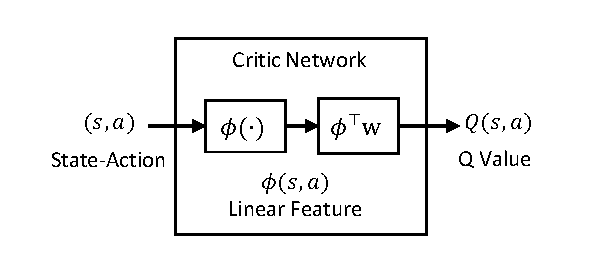
\includegraphics[width=230pt]{figs/Critic.pdf}
    \caption{Structure of a critic network contains a non-linear feature layer $\phi(\cdot)$ and a linear layer $\phi^{\top}w$.  }
    \label{fig:critic}
\end{figure}

\begin{algorithm}[!htb]
    \caption{Linear Feature Exploration Bonus}
    \label{alg:DE-AC}
    \begin{algorithmic}
        \STATE {\bfseries Input:} MDP $\mathcal{M} = <\mathcal{S},\mathcal{A},\mathcal{P},r,\gamma>$,
        \STATE Initialize critic $Q(s,a;\theta^Q)$ , actor $\pi(a|s;\theta^\pi)$
        \STATE Initialize replay buffer $D = \emptyset$, and temp buffer $T = \emptyset$.
        \STATE Initialize target network $Q^-= Q$, $\pi^-= \pi$.
        \STATE Initialize Feature Matrix $\Lambda = \lambda I$.
        \FOR{1 {\bfseries to} step\_number}
        \STATE Take action by $a \sim \pi(a|s;\theta^\pi)$
        \STATE Rollout data $s' \sim \mathcal{P}(s'|s,a)$,$r = r(s,a)$
        \STATE $T \leftarrow T\cup {<s,a>}$,$D \leftarrow D\cup {<s,a,r,s'>}$
        \IF  {$|T|=N_{temp}$}
        \STATE $\Phi \leftarrow [\phi(s_1,a_1),\phi(s_2,a_2),\cdots ]$ for each $s_i\in T$
        \STATE $\Lambda \leftarrow \Lambda + \Phi \Phi^\top $
        \ENDIF 
        \STATE Sample data batch $\{d=(s,a,r,s')\}$ from $D$
        \STATE $\Gamma = \beta [\phi(s,a)^\top(\Lambda)^{-1}\phi(s,a)]^{1/2}$
        \STATE $a'\sim \pi^-(a|s')$, $target  = r + \Gamma + Q^-(s',a')$
        \STATE $L^Q=\sum(Q(s,a)- target)^2$
        \STATE $\theta^Q \leftarrow \theta^Q - \alpha^Q\cdot\nabla_{\theta^Q} L^Q$
        \STATE $L^\pi=-\sum [\nabla\log(\pi(a|s)) \cdot Q(s,a)]$
        \STATE $\theta^\pi \leftarrow \theta^\pi -\alpha^\pi\cdot\nabla_{\theta^\pi} L^\pi$
        \STATE Soft update target network $Q'$ and $\pi'$
        \ENDFOR
     \end{algorithmic}
     \end{algorithm}

The calculation of LiFE bonus involves the operation of matrix inversion, which is numerically unstable. To solve this problem, we convert the data type from float32 to float64 when performing calculations related to the Feature Matrix. In addition, considering that the Feature Matrix $\Lambda$ is a symmetric matrix, we use symmetric eigenvalue decomposition $\Lambda = Q E Q^\top+\lambda I$ to make the calculations stable as follow:
\begin{equation}
    \begin{aligned}
    \phi^\top (\Lambda)^{-1}\phi &= \phi^\top (QEQ^\top+\lambda I)^{-1}\phi\\
    &= \phi^\top (Q(E+\lambda I)Q^\top)^{-1}\phi\\
    &= (Q^\top\phi)^\top (E+\lambda I)^{-1}(Q^\top\phi)
    \end{aligned}
\end{equation}

During the training process, the feature mapping part of the critical network is constantly changing. But recalculating the feature vector corresponding to all the data in the replay buffer and updating $\Lambda$ will cause too much overhead. As an approximation, we store the new transition data into a temporary buffet $T$ and update 
\[\Lambda \leftarrow \Lambda+ \sum \phi(T)\phi(T)^\top\]
 every $N_{temp}$ steps. The pseudo code of the entire algorithm is shown as Alg. \ref{alg:DE-AC} .

